% Drawing 154/08-6 -- folder 154, batch 08, archive page 150 (PDF page 151).
% Transcription: à gauche, un dessin : une droite fléchée $D_\rho$ coupée d'autres droites en un sommet $s$, l'orientation $\omega$ marquée par une petite flèche de rotation, et deux chemins en tirets (brun et vert) qui la longent, l'un fléché et marqué $D_{\rho,s,\omega}$ ; au-dessous, $\vec{\omega}_{D_\rho}$. À droite, un petit dessin : au sommet $\rho = \rho_D$, une flèche épaisse $\vec{a}_{s,\omega} = \vec{a}$, l'orientation $\varpi = \varpi_\rho$ et un contour en tirets fléché ; plus à droite, une arête $a = a_L$ entre deux faces $F_{\Delta'}$ et $F_{\Delta}$, avec les orientations $\omega_a$ et $\varpi_a$ ; au-dessous, une droite $L$ fléchée ($\omega_L$) passant par un sommet où est marquée l'orientation $\omega_s$
% Kind: arrowed line D_rho cut at a vertex s with orientation and two dashed paths; further local pictures. Method 2 (schematic redraw from the facsimile). Status: partial.
% Notes: Left: an arrowed line D_rho cut by other lines at a vertex s, the orientation omega as a small rotation arrow, and two dashed paths (brown and green) running along it, one arrowed and marked D_{rho,s,omega}. Further right, small ink sketches: a star of lines with an arrowed segment (vectors a_{s,rho}), two faces F_Delta', F_Delta on either side of a thick arrowed edge with lines through it, and an arrowed line L through a marked point with a small rotation arrow. Read from the page view; labels reduced to the main ones.
% Coordinates: 1 unit = 1 mm = 1/100 of the crop width (bbox in page fractions: [0.13, 0.14, 0.801, 0.316]).
% Redrawn by Claude (claude-opus-5-5), issue #73, 2026-11-07; not checked by a human; not compiled (no TeX in the session).
% Rights: reproduces part of the work -- behind RENDER_TRANSCRIPTS, never published by itself.
\documentclass[tikz,border=3pt]{standalone}
\usepackage{amsmath,amssymb}
\usetikzlibrary{patterns,arrows.meta}
\tikzset{Or/.style={orange!90!black}, Ye/.style={yellow!80!orange}, Lg/.style={green!60!black!70}, Dg/.style={green!45!black}, Br/.style={brown!80!black}, Rd/.style={red!85!black}, Bl/.style={blue!70!black}, Gy/.style={black!40}, pencil/.style={black!45}, struck/.style={black!35}, mark/.style={circle,draw,inner sep=1.3pt}, pt/.style={circle,fill,inner sep=0.9pt}, opt/.style={circle,draw,fill=white,inner sep=1.1pt}}
\begin{document}
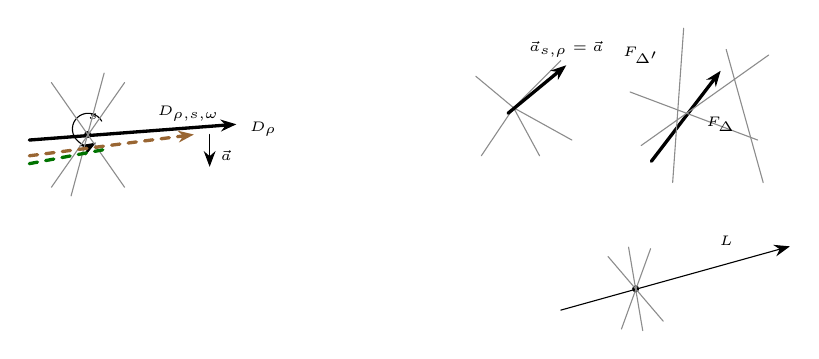
\begin{tikzpicture}[x=1mm,y=1mm,line cap=round,line join=round,font=\scriptsize]
\draw[-{Stealth[length=2mm]},very thick] (0.7,-14.2) -- (27,-12.2);
\node[inner sep=1pt] at (30.4,-12.8) {\tiny $D_\rho$};
\node[pt] at (8.1,-13.5) {};
\node[inner sep=1pt] at (8.8,-11.2) {\tiny $s$};
\draw[-{Stealth[length=2mm]}] (9.9,-11.8) arc[start angle=30, end angle=300, x radius=2, y radius=2];
\draw[pencil] (3.5,-20.2) -- (12.8,-6.9);
\draw[pencil] (6,-21.3) -- (10.2,-5.7);
\draw[pencil] (12.8,-20.2) -- (3.5,-6.9);
\draw[Br,dashed,very thick,-{Stealth[length=2mm]}] (0.7,-16.2) -- (21.6,-13.5);
\draw[Dg,dashed,very thick] (0.7,-17.2) -- (10.8,-15.3);
\node[inner sep=1pt] at (20.9,-10.8) {\tiny $D_{\rho,s,\omega}$};
\draw[-{Stealth[length=2mm]}] (23.6,-13.5) -- (23.6,-17.6);
\node[inner sep=1pt] at (25.7,-16.2) {\tiny $\vec a$};
\draw[pencil] (62.2,-10.1) -- (57.4,-6.1);
\draw[pencil] (62.2,-10.1) -- (68.2,-4.1);
\draw[pencil] (62.2,-10.1) -- (69.6,-14.2);
\draw[pencil] (62.2,-10.1) -- (58.1,-16.2);
\draw[pencil] (62.2,-10.1) -- (65.5,-16.2);
\draw[-{Stealth[length=2mm]},very thick] (61.5,-10.8) -- (68.9,-4.7);
\node[inner sep=1pt] at (68.9,-2.7) {\tiny $\vec a_{s,\rho}=\vec a$};
\draw[-{Stealth[length=2mm]},very thick] (79.7,-16.9) -- (88.5,-5.4);
\draw[pencil] (77,-8.1) -- (93.2,-14.2);
\draw[pencil] (83.8,-0) -- (82.4,-19.6);
\draw[pencil] (89.2,-2.7) -- (93.9,-19.6);
\draw[pencil] (78.4,-14.9) -- (94.6,-3.4);
\node[inner sep=1pt] at (78.4,-3.4) {\tiny $F_{\Delta'}$};
\node[inner sep=1pt] at (88.5,-12.2) {\tiny $F_\Delta$};
\draw[-{Stealth[length=2mm]}] (68.2,-35.8) -- (97.3,-27.7);
\node[pt] at (77.7,-33.1) {};
\draw[pencil] (78.6,-38.4) -- (76.8,-27.8);
\draw[pencil] (81.2,-37.2) -- (74.2,-29);
\draw[pencil] (75.9,-38.2) -- (79.6,-28);
\node[inner sep=1pt] at (89.2,-27) {\tiny $L$};
\end{tikzpicture}
\end{document}
